% Asset ID: FA21TFormulaeBoundaryEnrichmentTikZ-001
% Purpose: precise memory triangle for the t-formulae.
\documentclass[tikz,border=8pt]{standalone}
\usepackage{amsmath}
\usepackage{xcolor}
\usetikzlibrary{arrows.meta,calc}
\definecolor{Canvas}{HTML}{FAF9F6}\definecolor{Ivory}{HTML}{FFFFF0}\definecolor{LineSoft}{HTML}{E5E5EA}\definecolor{Accent}{HTML}{C5A059}\definecolor{Text}{HTML}{2C2C2E}
\begin{document}
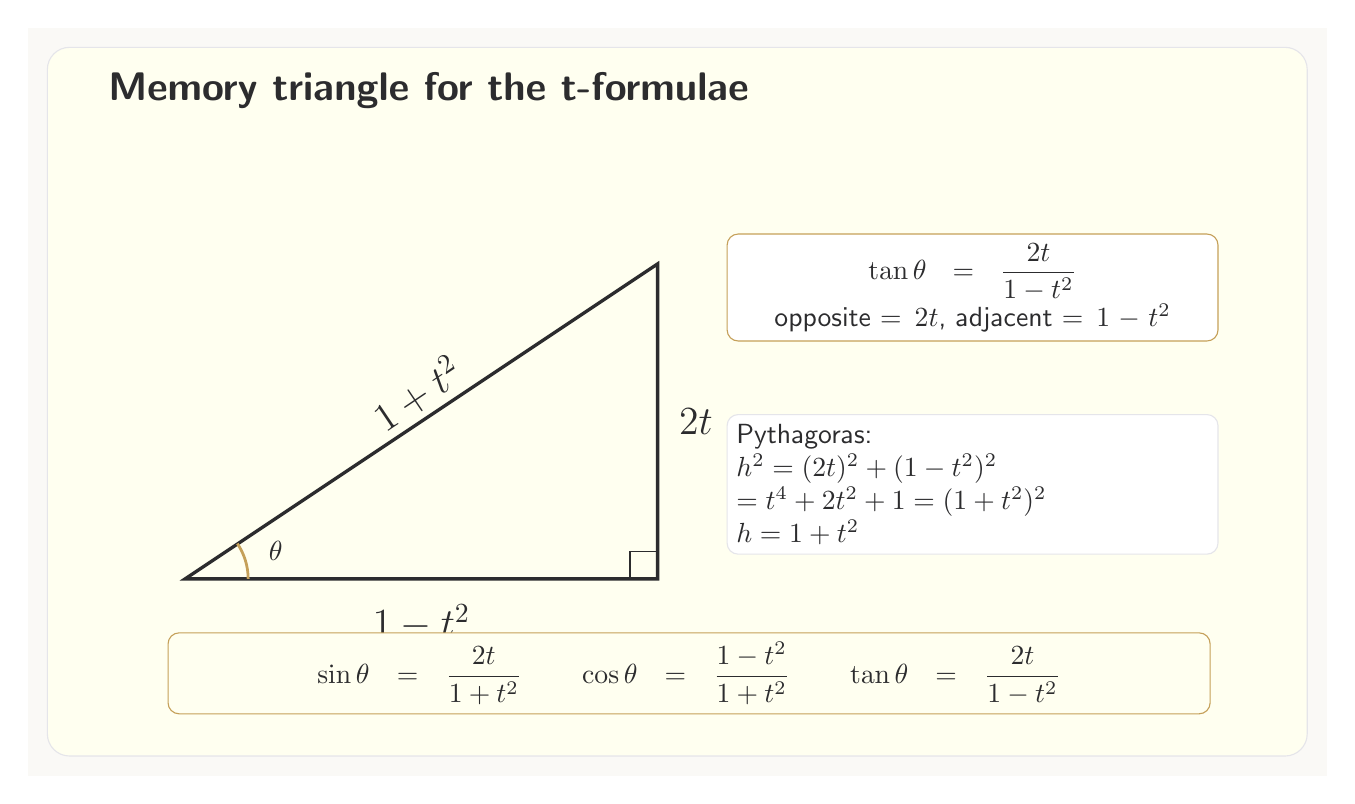
\begin{tikzpicture}[x=1cm,y=1cm,every node/.style={font=\sffamily,text=Text}]
\fill[Canvas] (-.5,-.5) rectangle (16,9);
\draw[LineSoft,fill=Ivory,rounded corners=8pt] (-.25,-.25) rectangle (15.75,8.75);
\node[anchor=west,font=\sffamily\bfseries\Large] at (.4,8.2) {Memory triangle for the t-formulae};
\coordinate (A) at (1.5,2); \coordinate (B) at (7.5,2); \coordinate (C) at (7.5,6);
\draw[Text,line width=1.2pt] (A)--(B)--(C)--cycle;
\draw[Text] ($(B)+(-.35,0)$)--++(0,.35)--++(.35,0);
\draw[Accent,line width=1pt] ($(A)+(.8,0)$) arc[start angle=0,end angle=34,radius=.8];
\node at ($(A)+(1.15,.35)$) {$\theta$};
\node[anchor=west,font=\sffamily\bfseries\Large] at ($(B)!.5!(C)+(.15,0)$) {$2t$};
\node[anchor=north,font=\sffamily\bfseries\Large] at ($(A)!.5!(B)+(0,-.2)$) {$1-t^2$};
\node[rotate=34,font=\sffamily\bfseries\Large] at ($(A)!.5!(C)+(-.05,.35)$) {$1+t^2$};
\node[draw=Accent,fill=white,rounded corners=4pt,align=center,text width=6cm] at (11.5,5.7) {$\displaystyle \tan\theta=\frac{2t}{1-t^2}$\\opposite $=2t$, adjacent $=1-t^2$};
\node[draw=LineSoft,fill=white,rounded corners=4pt,align=left,text width=6cm] at (11.5,3.2) {Pythagoras:\\$h^2=(2t)^2+(1-t^2)^2$\\$=t^4+2t^2+1=(1+t^2)^2$\\$h=1+t^2$};
\node[draw=Accent,fill=Ivory,rounded corners=4pt,align=center,text width=13cm] at (7.9,.8) {$\displaystyle \sin\theta=\frac{2t}{1+t^2}\qquad \cos\theta=\frac{1-t^2}{1+t^2}\qquad \tan\theta=\frac{2t}{1-t^2}$};
\end{tikzpicture}
\end{document}
